% SC2001 — Chapter 5: Greedy Algorithms
% No \documentclass — this file is \input/\include'd by main.tex.
\chapter{Greedy Algorithms}
\label{ch:greedy}
\begin{quote}
\emph{``Make the best local choice and never look back.''} --- The greedy motto. Sometimes it yields optimal solutions; often it does not. The craft lies in knowing which and proving it.
\end{quote}
\noindent\textbf{Prerequisites:} Asymptotic notation (Ch.~2), exchange arguments and induction (Ch.~1), priority queues and Union-Find (Ch.~3), basic graph terminology (Ch.~6 preview).

\section*{Learning Outcomes}
After this chapter you will be able to:
\begin{enumerate}[label=(L\arabic*)]
    \item describe the greedy paradigm and state the greedy-choice and optimal-substructure conditions;
    \item apply the exchange-argument template to prove correctness of a greedy algorithm;
    \item prove optimality of earliest-finish-time interval scheduling;
    \item construct Huffman codes and prove their optimality;
    \item state and apply the cut property to justify Kruskal's and Prim's MST algorithms;
    \item exhibit inputs where the greedy heuristic fails (coin change).
\end{enumerate}

\section{The Greedy Paradigm and the Exchange Argument}
\label{sec:greedy-paradigm}
A \emph{greedy} algorithm builds a solution incrementally, choosing at each step the locally best option according to some criterion, never reconsidering earlier choices.

\begin{figure}[h]\centering
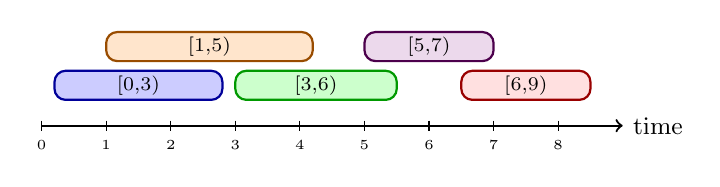
\begin{tikzpicture}[scale=0.82]
  \draw[->,thick] (0,0) -- (9,0) node[right,font=\small] {time};
  \foreach \x in {0,...,8} \draw (\x,0.08) -- (\x,-0.08) node[below,font=\tiny] {\x};
  \draw[fill=blue!20,draw=blue!60!black,thick,rounded corners] (0.2,0.4) rectangle (2.8,0.85) node[midway,font=\scriptsize] {[0,3)};
  \draw[fill=orange!20,draw=orange!60!black,thick,rounded corners] (1.0,1.0) rectangle (4.2,1.45) node[midway,font=\scriptsize] {[1,5)};
  \draw[fill=green!20,draw=green!60!black,thick,rounded corners] (3.0,0.4) rectangle (5.5,0.85) node[midway,font=\scriptsize] {[3,6)};
  \draw[fill=violet!15,draw=violet!60!black,thick,rounded corners] (5.0,1.0) rectangle (7.0,1.45) node[midway,font=\scriptsize] {[5,7)};
  \draw[fill=red!12,draw=red!60!black,thick,rounded corners] (6.5,0.4) rectangle (8.5,0.85) node[midway,font=\scriptsize] {[6,9)};
\end{tikzpicture}
\caption{Intervals on a timeline. Earliest finish (blue) leaves the most room --- scan left-to-right, no backtracking.}
\label{fig:timeline-intervals}
\end{figure}
\begin{definition}[Greedy choice \& optimal substructure]
An optimisation problem has the \emph{greedy-choice property} if a globally optimal solution can be assembled by making a locally optimal first choice and then solving the remaining subproblem optimally. It has \emph{optimal substructure} if an optimal solution contains optimal solutions to subproblems.
\end{definition}

Greedy is not universally correct; it requires both properties. Proofs of correctness almost always use an \emph{exchange argument}:

\begin{center}
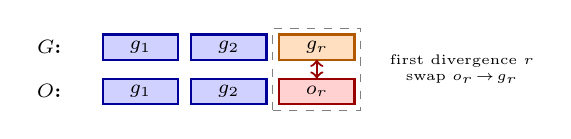
\begin{tikzpicture}[scale=0.80, every node/.style={font=\scriptsize}]
  \node[anchor=east,font=\scriptsize\bfseries] at (-0.2,0.75) {$G$:};
  \draw[fill=blue!18,draw=blue!60!black,thick] (0.3,0.55) rectangle (1.5,0.95) node[midway] {$g_1$};
  \draw[fill=blue!18,draw=blue!60!black,thick] (1.7,0.55) rectangle (2.9,0.95) node[midway] {$g_2$};
  \draw[fill=orange!25,draw=orange!70!black,thick] (3.1,0.55) rectangle (4.3,0.95) node[midway] {$g_r$};
  \node[anchor=east,font=\scriptsize\bfseries] at (-0.2,0.05) {$O$:};
  \draw[fill=blue!18,draw=blue!60!black,thick] (0.3,-0.15) rectangle (1.5,0.25) node[midway] {$g_1$};
  \draw[fill=blue!18,draw=blue!60!black,thick] (1.7,-0.15) rectangle (2.9,0.25) node[midway] {$g_2$};
  \draw[fill=red!18,draw=red!60!black,thick] (3.1,-0.15) rectangle (4.3,0.25) node[midway] {$o_r$};
  \draw[<->,thick,red!60!black] (3.7,0.55) -- (3.7,0.25);
  \draw[dashed,gray] (3.0,-0.25) rectangle (4.4,1.05);
  \node[font=\tiny,align=center] at (6.0,0.40) {first divergence $r$\\swap $o_r\!\to\!g_r$};
\end{tikzpicture}
\end{center}
Make $O$ look more like $G$ without hurting it --- the core of every exchange proof.

\begin{center}
\fbox{\parbox{0.92\linewidth}{%
\textbf{Exchange template.} Let $G$ be the greedy solution and $O$ an optimal solution that agrees with $G$ for as long as possible (first $k$ choices). Show the $(k{+}1)$st greedy choice can be exchanged into $O$ without worsening its value, obtaining $O'$ that agrees with $G$ one step further and remains optimal. By induction $G$ is optimal.
}}
\end{center}

Two recurring lemmas support the exchange: (i) \emph{greedy stays ahead} (after $k$ steps the greedy partial solution is at least as good as any competitor's), and (ii) \emph{cut/exchange} (swapping in the greedy element does not hurt feasibility or cost).

\section{Interval Scheduling: Earliest Finish Time}
\label{sec:interval-scheduling}

Given $n$ intervals $[s_i,f_i)$ (half-open), find a maximum-cardinality subset of pairwise compatible (non-overlapping) intervals.

\begin{lstlisting}[language=Python]
EarliestFinish(intervals):
  sort by finish time f_1 <= f_2 <= ... <= f_n
  S = empty; last = -inf
  for i = 1..n:
    if s_i >= last:  S.add(i); last = f_i
  return S
\end{lstlisting}

\begin{theorem}[Optimality of earliest finish]
EarliestFinish returns a maximum-size compatible set.
\end{theorem}
\begin{proof}[Exchange argument]
Let $G=\langle g_1,\dots,g_k\rangle$ be the greedy set in order of finish time and $O=\langle o_1,\dots,o_m\rangle$ an optimal set ordered the same way, chosen to maximise the longest common prefix with $G$. Let $r$ be the first index where they differ (or $r=k+1$ if $G$ is a prefix of $O$). If $r>k$ then $|G|\le|O|$ and, since $G$ is maximal, $|G|=|O|$. Otherwise $f_{g_r}\le f_{o_r}$ (greedy picks the earliest-finishing compatible interval) and $s_{o_{r+1}}\ge f_{o_r}\ge f_{g_r}$, so $O'=(O\setminus\{o_r\})\cup\{g_r\}$ is feasible and $|O'|=|O|$. $O'$ is optimal and agrees with $G$ one step further, contradicting maximality of $r$. Hence no such $r$ exists and $|G|=|O|$.
\end{proof}

The argument shows \emph{greedy stays ahead}: $f_{g_i}\le f_{o_i}$ for all $i\le\min(k,m)$. This invariant is the core of many greedy proofs---compare the $k$th greedy choice directly to the $k$th choice of any competitor.

{\sloppy
\begin{example}[Small instance]
Intervals $[1,4),[3,5),[0,6),[5,7),[8,9)$ sorted by finish are
$[1,4),[3,5),$ $[0,6),[5,7),[8,9)$. Greedy picks $[1,4),[5,7),[8,9)$
(size~3), optimal; $[1,4)\!\to\![0,6)$ cannot improve.
\end{example}\par}

Running time is $O(n\log n)$ for sorting plus $O(n)$ scanning. Variants (earliest start time, shortest interval, fewest conflicts) all fail---counterexamples are left as exercises.

\section{Huffman Coding}
\label{sec:huffman}

Given alphabet $C$ with frequencies $freq(c)>0$, find a binary \emph{prefix code} (no codeword is a prefix of another) minimising weighted path length $B(T)=\sum_{c}freq(c)\cdot d_T(c)$, where $d_T(c)$ is depth in the coding tree $T$.

Huffman's greedy rule: repeatedly merge the two lowest-frequency nodes.

\begin{lstlisting}[language=Python]
Huffman(C, freq):
  Q = min-heap of leaves by freq
  for i = 1 to |C|-1:
    x = Q.extractMin(); y = Q.extractMin()
    z = internal node with children x,y, freq(z)=freq(x)+freq(y)
    Q.insert(z)
  return Q.extractMin()  // root
\end{lstlisting}

\begin{figure}[h]\centering
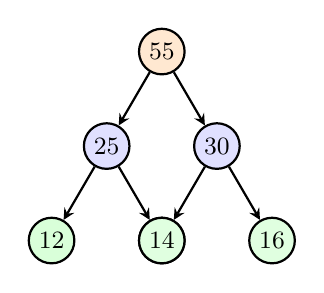
\begin{tikzpicture}[every node/.style={circle,draw,thick,inner sep=2pt,font=\small},
  level distance=12mm, sibling distance=14mm,
  edge from parent/.style={draw,-stealth,thick}]
\node[fill=orange!18] {55}
  child { node[fill=blue!12] {25} child { node[fill=green!15] {12} } child { node[fill=green!15] {13} } }
  child { node[fill=blue!12] {30} child { node[fill=green!12] {14} } child { node[fill=green!12] {16} } };
\end{tikzpicture}
\caption{Huffman tree sketch: internal labels are summed frequencies; leaves carry character frequencies (here $12,13,14,16$). The two smallest ($12,13$) are siblings at maximum depth---the greedy choice.}
\label{fig:huffman}
\end{figure}

\begin{lemma}[Sibling property]
There exists an optimal prefix tree in which the two least-frequent characters are siblings at maximum depth.
\end{lemma}
\paragraph{Numeric swap demo (before $\Delta$).} Rare $x$ (freq~12, depth~2) vs.\ frequent $a$ (freq~14, depth~3):
\begin{center}\small
\begin{tabular}{c|cc|c} & freq & depth & $freq\!\cdot\!depth$\\\hline $x$&12&2&24\\ $a$&14&3&42\\\hline\multicolumn{3}{c|}{before}&66\end{tabular}
$\to$
\begin{tabular}{c|cc|c} & freq & depth & $freq\!\cdot\!depth$\\\hline $x$&12&3&36\\ $a$&14&2&28\\\hline\multicolumn{3}{c|}{after}&64\end{tabular}
\end{center}
\begin{center}
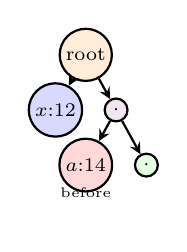
\begin{tikzpicture}[scale=0.70, every node/.style={circle,draw,thick,inner sep=1.5pt,font=\scriptsize}, level distance=10mm, sibling distance=11mm, edge from parent/.style={draw,-stealth,thick}]
  \node[fill=orange!15] at (0,0) {root} child { node[fill=blue!15] {$x$:12} } child { node[fill=violet!10] {$\cdot$} child { node[fill=red!15] {$a$:14} } child { node[fill=green!10] {$\cdot$} } };
  \node[draw=none,font=\tiny] at (0,-2.5) {before};
\end{tikzpicture}\hspace{4mm}
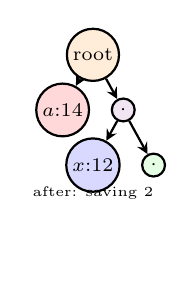
\begin{tikzpicture}[scale=0.70, every node/.style={circle,draw,thick,inner sep=1.5pt,font=\scriptsize}, level distance=10mm, sibling distance=11mm, edge from parent/.style={draw,-stealth,thick}]
  \node[fill=orange!15] at (0,0) {root} child { node[fill=red!15] {$a$:14} } child { node[fill=violet!10] {$\cdot$} child { node[fill=blue!15] {$x$:12} } child { node[fill=green!10] {$\cdot$} } };
  \node[draw=none,font=\tiny] at (0,-2.5) {after: saving $2$};
\end{tikzpicture}
\end{center}
Saving $=(14-12)(3-2)=2\ge0$; in general $\Delta=(freq(a)-freq(x))(d(a)-d(x))$.

\begin{proof}[Exchange]
Take an optimal tree $T$ and let $x,y$ be the two least-frequent characters. Let $a,b$ be siblings at maximum depth in $T$. If $\{x,y\}=\{a,b\}$ we are done. Otherwise swap $x$ with $a$ (and $y$ with $b$ if needed). Since $freq(x)\le freq(a)$ and $d(x)\le d(a)$ cannot both be reversed, each swap does not increase $B(T)$: $\Delta = (freq(a)-freq(x))(d(a)-d(x))\ge 0$ cost is not raised. The resulting tree is optimal with $x,y$ as deepest siblings.
\end{proof}

\begin{theorem}[Huffman optimality]
Huffman produces an optimal prefix code.
\end{theorem}
\begin{proof}[Induction + exchange]
Induction on $|C|=n$. Base $n=2$ trivial. For $n>1$, let $x,y$ be the two smallest frequencies merged into $z$ with $freq(z)=freq(x)+freq(y)$. Let $T'$ be the optimal tree for $C'=(C\setminus\{x,y\})\cup\{z\}$ given by induction (Huffman on $C'$). Expand $z$ into $x,y$ to get $T$; then $B(T)=B(T')+freq(x)+freq(y)$. If some tree $T^*$ for $C$ had $B(T^*)<B(T)$, transform $T^*$ by the Lemma so $x,y$ are siblings, contract them to $z$ to get $T^*_0$ for $C'$ with $B(T^*_0)=B(T^*)-freq(x)-freq(y)<B(T')$, contradicting optimality of $T'$.
\end{proof}
Complexity is $O(n\log n)$ with a heap. Decoding is unambiguous precisely because the code is prefix-free---the tree path is followed until a leaf is reached. Optimal merging and the structure of prefix codes both hinge on the same exchange idea.

\begin{remark}
Kraft's inequality $\sum_c 2^{-d_T(c)}\le 1$ characterises feasible prefix-code lengths. Huffman achieves minimum $\sum freq(c)d_T(c)$, i.e.\ minimum redundancy above entropy $H=-\sum p_c\log p_c$.
\end{remark}

\section{Minimum Spanning Trees: The Cut Property}
\label{sec:mst}

Let $G=(V,E)$ be connected, undirected, with distinct edge weights $w(e)$ (ties broken arbitrarily). A \emph{spanning tree} minimises total weight among all spanning trees if it is an MST.

Picture a cut first: partition $V$ into $S$ and $V\setminus S$ (dashed bubble). Which crossing edge must every MST take? The lightest one.

\begin{figure}[h]\centering
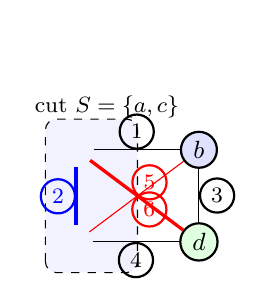
\begin{tikzpicture}[scale=0.78, every node/.style={circle,draw,thick,inner sep=2pt,font=\small}]
  \node[fill=blue!12] (a) at (0,1.5) {$a$}; \node[fill=blue!12] (b) at (2,1.5) {$b$};
  \node[fill=green!12] (c) at (0,0) {$c$}; \node[fill=green!12] (d) at (2,0) {$d$};
  \draw[dashed,rounded corners,fill=blue!5] (-0.5,-0.5) rectangle (1,2);
  \node[draw=none,font=\footnotesize] at (0.5,2.2) {cut $S=\{a,c\}$};
  \draw (a) -- node[above,font=\footnotesize] {1} (b);
  \draw[ultra thick,blue] (a) -- node[left,font=\footnotesize] {2} (c);
  \draw (c) -- node[below,font=\footnotesize] {4} (d);
  \draw (b) -- node[right,font=\footnotesize] {3} (d);
  \draw[red,very thick] (a) -- node[above right,font=\footnotesize] {5} (d);
  \draw[red] (c) -- node[below right,font=\footnotesize] {6} (b);
\end{tikzpicture}
\caption{Cut $(S,V\setminus S)$, $S=\{a,c\}$. Crossing edges weigh $1,3,5,6$; the lightest (weight~1) must be in every MST (cut property below).}
\label{fig:mst-cut}
\end{figure}

\begin{definition}[Cut property]
For any cut $(S,V\setminus S)$, the minimum-weight edge crossing the cut belongs to every MST.
\end{definition}

\begin{proof}[Exchange]
Let $e=(u,v)$ be the lightest edge crossing $(S,V\setminus S)$ and suppose some MST $T$ omits $e$. Adding $e$ to $T$ creates a unique cycle $C$, which must cross the cut in another edge $f\neq e$. Since $w(e)<w(f)$, $T'=(T\setminus\{f\})\cup\{e\}$ is a spanning tree lighter than $T$---contradiction. Hence $e\in T$.
\end{proof}

Both classic algorithms are greedy instantiations of this property.

\begin{lstlisting}[language=Python]
Kruskal(V,E,w):
  sort E by w ascending; make Union-Find on V
  T = empty
  for e=(u,v) in sorted E:
    if Find(u) != Find(v): T.add(e); Union(u,v)  % Find=already connected? Union=merge
  return T
\end{lstlisting}
Each edge added by Kruskal is the lightest crossing the cut $(C,V\setminus C)$ where $C$ is its component before the union.

\begin{lstlisting}[language=Python]
Prim(V,E,w, r):
  S={r}; T=empty; PQ = edges leaving S keyed by w  % key = cheapest edge leaving $S$
  while S != V:
    e=(u,v)=PQ.extractMin() with u in S, v not in S
    T.add(e); S.add(v); insert edges from v to V\S into PQ
  return T
\end{lstlisting}
Each edge added by Prim is exactly the minimum edge of cut $(S,V\setminus S)$.

Correctness of both follows immediately from the cut property: every edge they add is forced into every MST, so the final tree is contained in all MSTs and hence is one itself. Kruskal runs in $O(|E|\log|E|)$ (sorting dominates); Prim with a binary heap is $O(|E|\log|V|)$, $O(|E|+|V|\log|V|)$ with a Fibonacci heap. The cycle property (heaviest edge on any cycle is never in any MST) is dual and also proved by exchange.

\section{When Greedy Fails: Coin Change}
\label{sec:coin-change}

Given denominations $D=\{d_1<\dots<d_k\}$ and amount $A$, minimise number of coins. The greedy rule---repeatedly take the largest $d_i\le$ remaining amount---is optimal for canonical systems (e.g.\ US coins $\{1,5,10,25\}$) but not in general.

\begin{example}[Counterexample]
$D=\{1,3,4\}$, $A=6$. Greedy picks $4+1+1$ (3 coins) while $3+3$ uses 2 coins. For $D=\{1,10,25\}$, $A=30$: greedy gives $25+1+1+1+1+1$ (6 coins) vs.\ $10+10+10$ (3 coins).
\end{example}

The DP table for $D=\{1,3,4\}$, $A=6$ illustrates the fix:
\begin{center}
\begin{tabular}{c|ccccccc}
$x$ & 0 & 1 & 2 & 3 & 4 & 5 & 6\\\hline
$dp[x]$ & 0 & 1 & 2 & 1 & 1 & 2 & 2\\
choice & -- & 1 & 1 & 3 & 4 & 1+4 & 3+3
\end{tabular}
\end{center}
Greedy is myopic: taking $4$ at $x=6$ forces two $1$s, while $dp$ considers all predecessors $x-d_i$.
More generally, no fixed greedy order works for all $D$. The problem is solved optimally by dynamic programming in $O(kA)$:
\[ dp[0]=0,\quad dp[x]=\min_{d_i\le x}\{1+dp[x-d_i]\}. \]
The failure illustrates the missing greedy-choice property: a locally optimal coin can block a globally better combination.

\section{Exercises}
\label{sec:greedy-exercises}

\begin{enumerate}[label=E\arabic*.]
    \item \textbf{Interval variants that fail.} Give counterexamples showing that (a) earliest start time, (b) shortest interval first, and (c) fewest conflicts first are \emph{not} optimal for interval scheduling.
    \item \textbf{Huffman trace.} For frequencies $\{5,9,12,13,16,45\}$, simulate Huffman step-by-step, draw the final tree, compute $B(T)$, and verify the average code length against the entropy lower bound.
    \item \textbf{Coin-change classification.} Prove that greedy is optimal for $D=\{1,5,10,25\}$ (US coins without the half-dollar). Then find the smallest $A$ where greedy fails for $D=\{1,3,4\}$ and prove $dp$ above is correct.
    \item \textbf{Cut/cycle duality.} Prove the \emph{cycle property}: if $e$ is the maximum-weight edge on some cycle, no MST contains $e$. Deduce that the MST is unique when all edge weights are distinct.
    \item \textbf{Scheduling with deadlines.} Each job has duration $t_i$ and deadline $d_i$. The greedy order by earliest deadline minimises maximum lateness $L_{\max}=\max_i(f_i-d_i)$ where $f_i$ is completion time. Prove optimality via an exchange argument (adjacent swap).
\end{enumerate}

\section*{Chapter Notes}
Huffman (1952), Kruskal/Prim (1956--57): matroid optimisation; interval scheduling $\to$ weighted (Ch.\,7 DP). U.S.\ coins canonical---Pearson (2005). See matroids/greedoids.

